% Options for packages loaded elsewhere
\PassOptionsToPackage{unicode}{hyperref}
\PassOptionsToPackage{hyphens}{url}
\PassOptionsToPackage{dvipsnames,svgnames,x11names}{xcolor}
%
\documentclass[
  letterpaper,
  DIV=11,
  numbers=noendperiod]{scrartcl}

\usepackage{amsmath,amssymb}
\usepackage{iftex}
\ifPDFTeX
  \usepackage[T1]{fontenc}
  \usepackage[utf8]{inputenc}
  \usepackage{textcomp} % provide euro and other symbols
\else % if luatex or xetex
  \usepackage{unicode-math}
  \defaultfontfeatures{Scale=MatchLowercase}
  \defaultfontfeatures[\rmfamily]{Ligatures=TeX,Scale=1}
\fi
\usepackage{lmodern}
\ifPDFTeX\else  
    % xetex/luatex font selection
\fi
% Use upquote if available, for straight quotes in verbatim environments
\IfFileExists{upquote.sty}{\usepackage{upquote}}{}
\IfFileExists{microtype.sty}{% use microtype if available
  \usepackage[]{microtype}
  \UseMicrotypeSet[protrusion]{basicmath} % disable protrusion for tt fonts
}{}
\makeatletter
\@ifundefined{KOMAClassName}{% if non-KOMA class
  \IfFileExists{parskip.sty}{%
    \usepackage{parskip}
  }{% else
    \setlength{\parindent}{0pt}
    \setlength{\parskip}{6pt plus 2pt minus 1pt}}
}{% if KOMA class
  \KOMAoptions{parskip=half}}
\makeatother
\usepackage{xcolor}
\usepackage[left=1in,right=1in,top=1in,bottom=1in]{geometry}
\setlength{\emergencystretch}{3em} % prevent overfull lines
\setcounter{secnumdepth}{-\maxdimen} % remove section numbering
% Make \paragraph and \subparagraph free-standing
\makeatletter
\ifx\paragraph\undefined\else
  \let\oldparagraph\paragraph
  \renewcommand{\paragraph}{
    \@ifstar
      \xxxParagraphStar
      \xxxParagraphNoStar
  }
  \newcommand{\xxxParagraphStar}[1]{\oldparagraph*{#1}\mbox{}}
  \newcommand{\xxxParagraphNoStar}[1]{\oldparagraph{#1}\mbox{}}
\fi
\ifx\subparagraph\undefined\else
  \let\oldsubparagraph\subparagraph
  \renewcommand{\subparagraph}{
    \@ifstar
      \xxxSubParagraphStar
      \xxxSubParagraphNoStar
  }
  \newcommand{\xxxSubParagraphStar}[1]{\oldsubparagraph*{#1}\mbox{}}
  \newcommand{\xxxSubParagraphNoStar}[1]{\oldsubparagraph{#1}\mbox{}}
\fi
\makeatother

\usepackage{color}
\usepackage{fancyvrb}
\newcommand{\VerbBar}{|}
\newcommand{\VERB}{\Verb[commandchars=\\\{\}]}
\DefineVerbatimEnvironment{Highlighting}{Verbatim}{commandchars=\\\{\}}
% Add ',fontsize=\small' for more characters per line
\usepackage{framed}
\definecolor{shadecolor}{RGB}{241,243,245}
\newenvironment{Shaded}{\begin{snugshade}}{\end{snugshade}}
\newcommand{\AlertTok}[1]{\textcolor[rgb]{0.68,0.00,0.00}{#1}}
\newcommand{\AnnotationTok}[1]{\textcolor[rgb]{0.37,0.37,0.37}{#1}}
\newcommand{\AttributeTok}[1]{\textcolor[rgb]{0.40,0.45,0.13}{#1}}
\newcommand{\BaseNTok}[1]{\textcolor[rgb]{0.68,0.00,0.00}{#1}}
\newcommand{\BuiltInTok}[1]{\textcolor[rgb]{0.00,0.23,0.31}{#1}}
\newcommand{\CharTok}[1]{\textcolor[rgb]{0.13,0.47,0.30}{#1}}
\newcommand{\CommentTok}[1]{\textcolor[rgb]{0.37,0.37,0.37}{#1}}
\newcommand{\CommentVarTok}[1]{\textcolor[rgb]{0.37,0.37,0.37}{\textit{#1}}}
\newcommand{\ConstantTok}[1]{\textcolor[rgb]{0.56,0.35,0.01}{#1}}
\newcommand{\ControlFlowTok}[1]{\textcolor[rgb]{0.00,0.23,0.31}{\textbf{#1}}}
\newcommand{\DataTypeTok}[1]{\textcolor[rgb]{0.68,0.00,0.00}{#1}}
\newcommand{\DecValTok}[1]{\textcolor[rgb]{0.68,0.00,0.00}{#1}}
\newcommand{\DocumentationTok}[1]{\textcolor[rgb]{0.37,0.37,0.37}{\textit{#1}}}
\newcommand{\ErrorTok}[1]{\textcolor[rgb]{0.68,0.00,0.00}{#1}}
\newcommand{\ExtensionTok}[1]{\textcolor[rgb]{0.00,0.23,0.31}{#1}}
\newcommand{\FloatTok}[1]{\textcolor[rgb]{0.68,0.00,0.00}{#1}}
\newcommand{\FunctionTok}[1]{\textcolor[rgb]{0.28,0.35,0.67}{#1}}
\newcommand{\ImportTok}[1]{\textcolor[rgb]{0.00,0.46,0.62}{#1}}
\newcommand{\InformationTok}[1]{\textcolor[rgb]{0.37,0.37,0.37}{#1}}
\newcommand{\KeywordTok}[1]{\textcolor[rgb]{0.00,0.23,0.31}{\textbf{#1}}}
\newcommand{\NormalTok}[1]{\textcolor[rgb]{0.00,0.23,0.31}{#1}}
\newcommand{\OperatorTok}[1]{\textcolor[rgb]{0.37,0.37,0.37}{#1}}
\newcommand{\OtherTok}[1]{\textcolor[rgb]{0.00,0.23,0.31}{#1}}
\newcommand{\PreprocessorTok}[1]{\textcolor[rgb]{0.68,0.00,0.00}{#1}}
\newcommand{\RegionMarkerTok}[1]{\textcolor[rgb]{0.00,0.23,0.31}{#1}}
\newcommand{\SpecialCharTok}[1]{\textcolor[rgb]{0.37,0.37,0.37}{#1}}
\newcommand{\SpecialStringTok}[1]{\textcolor[rgb]{0.13,0.47,0.30}{#1}}
\newcommand{\StringTok}[1]{\textcolor[rgb]{0.13,0.47,0.30}{#1}}
\newcommand{\VariableTok}[1]{\textcolor[rgb]{0.07,0.07,0.07}{#1}}
\newcommand{\VerbatimStringTok}[1]{\textcolor[rgb]{0.13,0.47,0.30}{#1}}
\newcommand{\WarningTok}[1]{\textcolor[rgb]{0.37,0.37,0.37}{\textit{#1}}}

\providecommand{\tightlist}{%
  \setlength{\itemsep}{0pt}\setlength{\parskip}{0pt}}\usepackage{longtable,booktabs,array}
\usepackage{calc} % for calculating minipage widths
% Correct order of tables after \paragraph or \subparagraph
\usepackage{etoolbox}
\makeatletter
\patchcmd\longtable{\par}{\if@noskipsec\mbox{}\fi\par}{}{}
\makeatother
% Allow footnotes in longtable head/foot
\IfFileExists{footnotehyper.sty}{\usepackage{footnotehyper}}{\usepackage{footnote}}
\makesavenoteenv{longtable}
\usepackage{graphicx}
\makeatletter
\def\maxwidth{\ifdim\Gin@nat@width>\linewidth\linewidth\else\Gin@nat@width\fi}
\def\maxheight{\ifdim\Gin@nat@height>\textheight\textheight\else\Gin@nat@height\fi}
\makeatother
% Scale images if necessary, so that they will not overflow the page
% margins by default, and it is still possible to overwrite the defaults
% using explicit options in \includegraphics[width, height, ...]{}
\setkeys{Gin}{width=\maxwidth,height=\maxheight,keepaspectratio}
% Set default figure placement to htbp
\makeatletter
\def\fps@figure{htbp}
\makeatother

\usepackage{booktabs}
\usepackage{longtable}
\usepackage{array}
\usepackage{multirow}
\usepackage{wrapfig}
\usepackage{float}
\usepackage{colortbl}
\usepackage{pdflscape}
\usepackage{tabu}
\usepackage{threeparttable}
\usepackage{threeparttablex}
\usepackage[normalem]{ulem}
\usepackage{makecell}
\usepackage{xcolor}
\usepackage{fvextra}
\DefineVerbatimEnvironment{Highlighting}{Verbatim}{breaklines,commandchars=\\\{\}}
\DefineVerbatimEnvironment{OutputCode}{Verbatim}{breaklines,commandchars=\\\{\}}
\KOMAoption{captions}{tableheading}
\makeatletter
\@ifpackageloaded{caption}{}{\usepackage{caption}}
\AtBeginDocument{%
\ifdefined\contentsname
  \renewcommand*\contentsname{Table of contents}
\else
  \newcommand\contentsname{Table of contents}
\fi
\ifdefined\listfigurename
  \renewcommand*\listfigurename{List of Figures}
\else
  \newcommand\listfigurename{List of Figures}
\fi
\ifdefined\listtablename
  \renewcommand*\listtablename{List of Tables}
\else
  \newcommand\listtablename{List of Tables}
\fi
\ifdefined\figurename
  \renewcommand*\figurename{Figure}
\else
  \newcommand\figurename{Figure}
\fi
\ifdefined\tablename
  \renewcommand*\tablename{Table}
\else
  \newcommand\tablename{Table}
\fi
}
\@ifpackageloaded{float}{}{\usepackage{float}}
\floatstyle{ruled}
\@ifundefined{c@chapter}{\newfloat{codelisting}{h}{lop}}{\newfloat{codelisting}{h}{lop}[chapter]}
\floatname{codelisting}{Listing}
\newcommand*\listoflistings{\listof{codelisting}{List of Listings}}
\makeatother
\makeatletter
\makeatother
\makeatletter
\@ifpackageloaded{caption}{}{\usepackage{caption}}
\@ifpackageloaded{subcaption}{}{\usepackage{subcaption}}
\makeatother

\ifLuaTeX
  \usepackage{selnolig}  % disable illegal ligatures
\fi
\usepackage{bookmark}

\IfFileExists{xurl.sty}{\usepackage{xurl}}{} % add URL line breaks if available
\urlstyle{same} % disable monospaced font for URLs
\hypersetup{
  pdftitle={IDK: A Statistical Analysis of Palm Beach County Election Votes in 2000},
  pdfauthor={Sydney Weisberg and Molly Daniel},
  colorlinks=true,
  linkcolor={blue},
  filecolor={Maroon},
  citecolor={Blue},
  urlcolor={Blue},
  pdfcreator={LaTeX via pandoc}}


\title{IDK: A Statistical Analysis of Palm Beach County Election Votes
in 2000}
\author{Sydney Weisberg and Molly Daniel}
\date{Invalid Date}

\begin{document}
\maketitle


\section{Introduction}\label{introduction}

\section{Data Description}\label{data-description}

The election data consists of the numbers of votes for Buchanan and Bush
in all 67 counties in Florida.

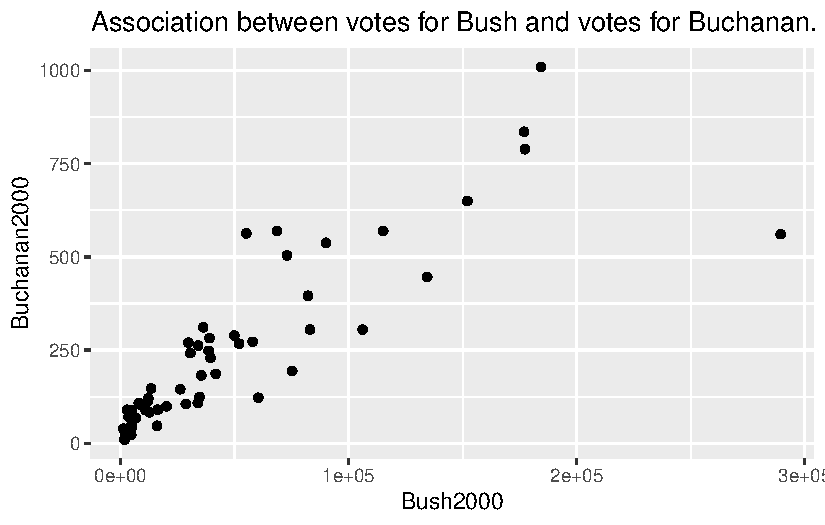
\includegraphics{case_study_1_files/figure-pdf/warning-FALSE-1.pdf}

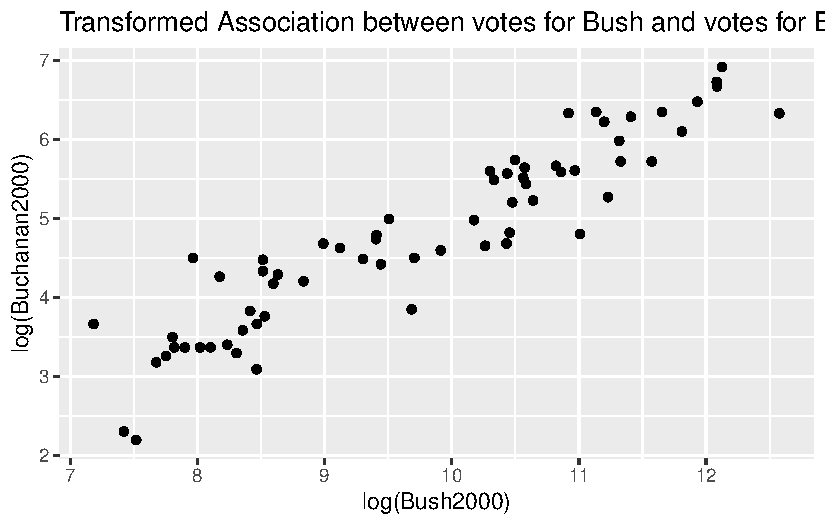
\includegraphics{case_study_1_files/figure-pdf/warning-FALSE-2.pdf}

\section{Modeling Process}\label{modeling-process}

In order to create a model, we first observed a relationship in the
scatter plot showing the votes for Buchanan and Bush in each of the
Florida counties. From this, we noticed data clustering occurring in the
bottom left corner of the scatter plot. In order to expand the scale, we
applied a log transformation to both the Buchanan and Bush votes,
revealing a multiplicative relationship between the two.

Let \(buchanan_i\) denote the number of votes cast for Buchanan in
county \(i\) and \(bush_i\) denote the number of votes cast for Bush in
Florida county \(i\) during the U.S. presidential election of November
7, 2000. Our final linear regression model for the mean is
\(E[log(buchanan_i) | log(bush_i)] = \beta_0 + \beta_1\log(bush_i).\) We
fit our sample data to this model, and found estimates for the
coefficients.

\begin{table}[H]
\centering
\begin{tabular}[t]{lcccc}
\toprule
  & Estimate & Std. Error & t value & Pr(>|t|)\\
\midrule
(Intercept) & -2.34 & 0.35 & -6.61 & 0\\
log(Bush2000) & 0.73 & 0.04 & 20.32 & 0\\
\bottomrule
\end{tabular}
\end{table}

Our sample intercept, \(\hat{\beta_0}\), is -2.34149 with a standard
error of 0.35442. Our sample slope, \(\hat{\beta_1}\), is 0.73096 with a
standard error of 0.03597. Both coefficients have a p value less than
0.05, making them statistically significant. So our fitted model is
\(\widehat{\log(buchanan_i)} = -2.34149 + 0.73096\log(bush_i).\)

Point Estimate = e\^{}6.384143 = 592.376848042

Prediction Interval = (e\^{}5.524656, e\^{}7.24363) = (250.8, 1399.164)

This means that we are 95\% confident that the number of votes cast for
Buchanan in the U.S. presidential election of November 7, 2000 when the
number of votes cast for Bush is 152846 (the reported number of votes
for Bush in Palm Beach county) is between 250.8 and 1399.164 votes.

\section{Conclusion}\label{conclusion}

Since the 3407 votes for Buchanan in Palm Beach County in the 2000
election falls outside of our prediction interval of 250.8 to 1399.164
where Bush receives 15,2846 votes, we can conclude that it is likely
that there is some external factor impacting the votes of the residents
in Palm Beach. One limitation of this analysis is the lack of
information regarding the sociopolitical climate of Palm Beach County in
2020. We do not know the demographic breakdown of the county. If there
were a higher percentage of centrists who would vote for a member of the
Reform Party in 2020 then that could explain the abnormal amount of
Buchanan votes. Additionally, we don't know what campaigning was like in
Palm Beach County. There could have been additional campaigns for
Buchanan there that caused a vote increase particularly in that county.
Based on the assumption that some of the votes cast for Buchanan in Palm
Beach were actually intended to be votes for Gore, we make a
generalization that there are more Democratic voters in Palm Beach
County than represented in our data. Without the cultural knowledge of
the environment where the data comes from, we can't be fully confident
that our model is a good fit for the data.

\section{R Appendix}\label{r-appendix}

\begin{Shaded}
\begin{Highlighting}[]
\CommentTok{\# Importing relevant packages}
\FunctionTok{library}\NormalTok{(tidyverse)}
\FunctionTok{library}\NormalTok{(Sleuth2)}
\FunctionTok{library}\NormalTok{(broom)}
\FunctionTok{library}\NormalTok{(kableExtra) }

\CommentTok{\# Importing election data from the textbook}
\NormalTok{election }\OtherTok{\textless{}{-}}\NormalTok{ Sleuth2}\SpecialCharTok{::}\NormalTok{ex0825}

\CommentTok{\# Removing the extreme Palm Beach observation}
\NormalTok{election\_wo\_pb }\OtherTok{\textless{}{-}}\NormalTok{ election }\SpecialCharTok{|\textgreater{}} \FunctionTok{filter}\NormalTok{(County }\SpecialCharTok{!=} \StringTok{"Palm Beach"}\NormalTok{)}

\CommentTok{\# Displaying an untransformed scatter plot between Bush and Buchanan votes}
\NormalTok{election\_wo\_pb }\SpecialCharTok{|\textgreater{}} \FunctionTok{ggplot}\NormalTok{(}\FunctionTok{aes}\NormalTok{(}\AttributeTok{x =}\NormalTok{ Bush2000, }\AttributeTok{y =}\NormalTok{ Buchanan2000)) }\SpecialCharTok{+} \FunctionTok{geom\_point}\NormalTok{() }\SpecialCharTok{+} \FunctionTok{ggtitle}\NormalTok{(}\StringTok{"Association between votes for Bush and votes for Buchanan."}\NormalTok{)}
\end{Highlighting}
\end{Shaded}

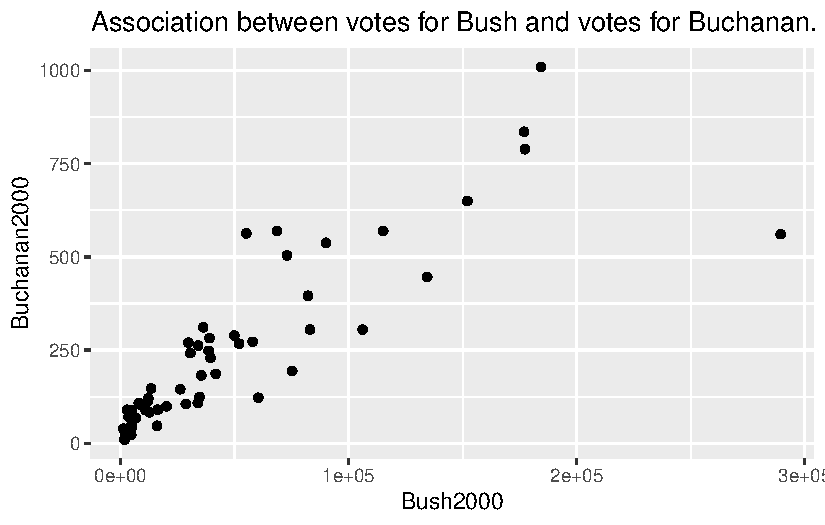
\includegraphics{case_study_1_files/figure-pdf/unnamed-chunk-3-1.pdf}

\begin{Shaded}
\begin{Highlighting}[]
\CommentTok{\# Displaying a doubly transformed scatter plot between Bush and Buchanan votes}
\NormalTok{election\_wo\_pb }\SpecialCharTok{|\textgreater{}} \FunctionTok{ggplot}\NormalTok{(}\FunctionTok{aes}\NormalTok{(}\AttributeTok{x =} \FunctionTok{log}\NormalTok{(Bush2000), }\AttributeTok{y =} \FunctionTok{log}\NormalTok{(Buchanan2000))) }\SpecialCharTok{+} \FunctionTok{geom\_point}\NormalTok{() }\SpecialCharTok{+} \FunctionTok{ggtitle}\NormalTok{(}\StringTok{"Transformed Association between votes for Bush and votes for Buchanan."}\NormalTok{)}
\end{Highlighting}
\end{Shaded}

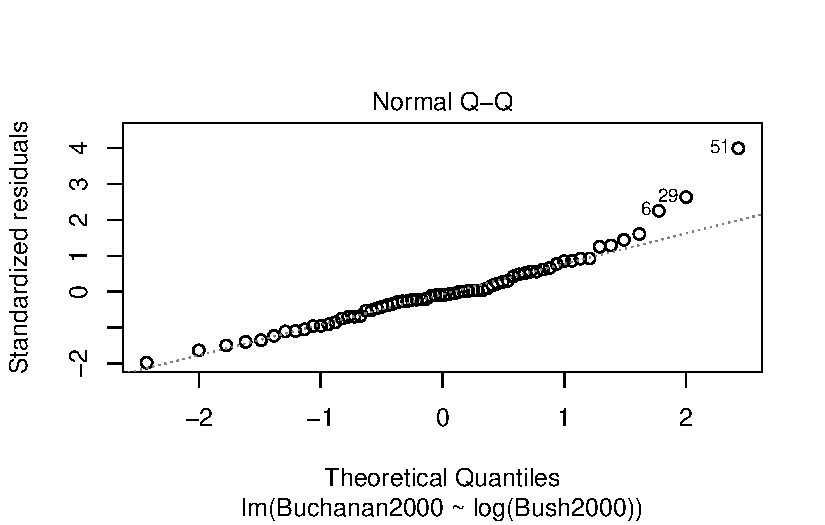
\includegraphics{case_study_1_files/figure-pdf/unnamed-chunk-3-2.pdf}

\begin{Shaded}
\begin{Highlighting}[]
\CommentTok{\# Testing transformations to determine the best fit for the model}

\CommentTok{\# Untransformed model}
\NormalTok{untransformed }\OtherTok{\textless{}{-}} \FunctionTok{lm}\NormalTok{(Buchanan2000 }\SpecialCharTok{\textasciitilde{}}\NormalTok{ Bush2000, }\AttributeTok{data =}\NormalTok{ election\_wo\_pb)}
\FunctionTok{plot}\NormalTok{(untransformed)}
\end{Highlighting}
\end{Shaded}

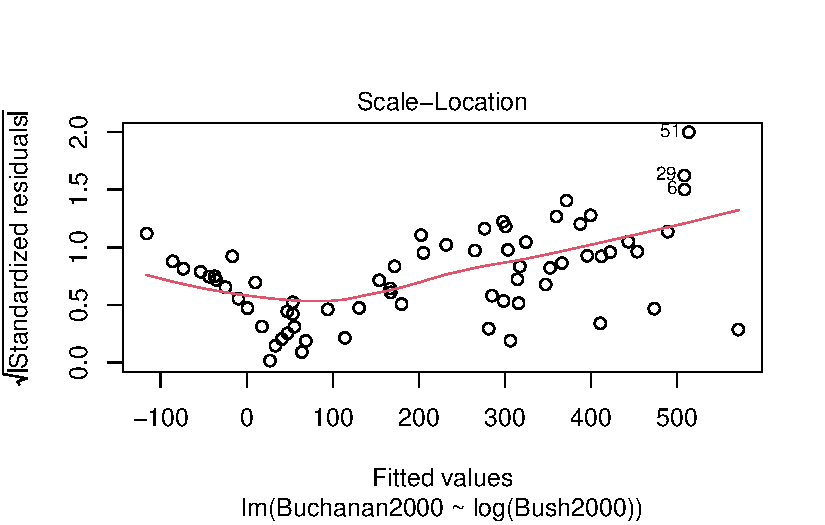
\includegraphics{case_study_1_files/figure-pdf/unnamed-chunk-3-3.pdf}

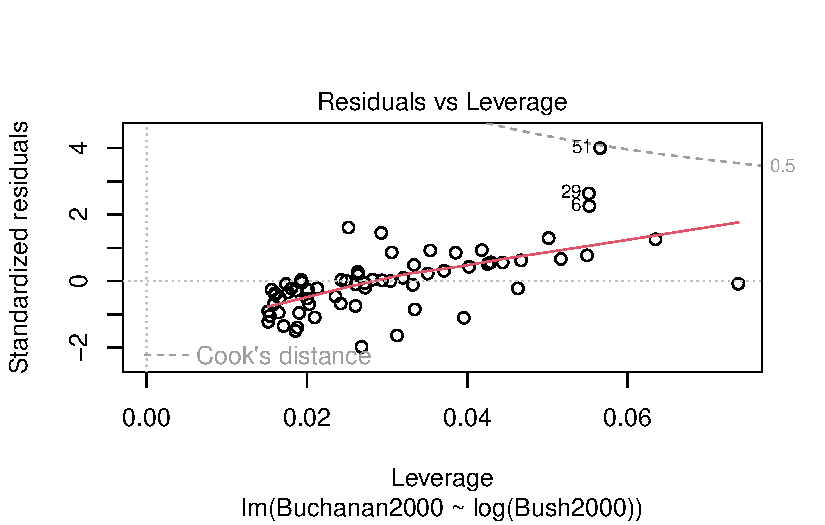
\includegraphics{case_study_1_files/figure-pdf/unnamed-chunk-3-4.pdf}

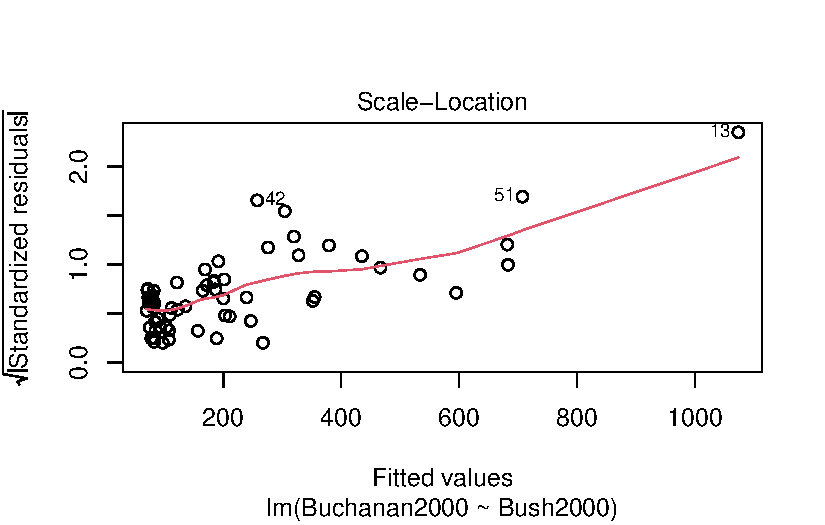
\includegraphics{case_study_1_files/figure-pdf/unnamed-chunk-3-5.pdf}

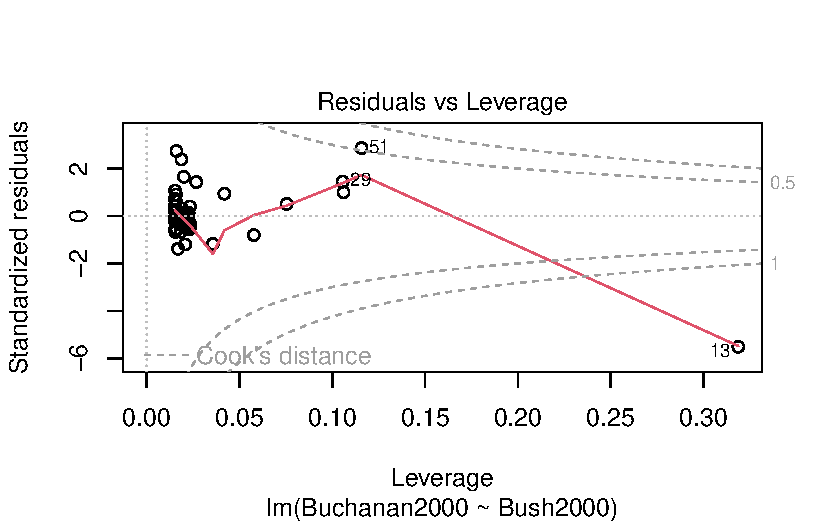
\includegraphics{case_study_1_files/figure-pdf/unnamed-chunk-3-6.pdf}

\begin{Shaded}
\begin{Highlighting}[]
\CommentTok{\# Model with a logarithmic explanatory variable transformation}
\NormalTok{xtransformed }\OtherTok{\textless{}{-}} \FunctionTok{lm}\NormalTok{(Buchanan2000 }\SpecialCharTok{\textasciitilde{}} \FunctionTok{log}\NormalTok{(Bush2000), }\AttributeTok{data =}\NormalTok{ election\_wo\_pb)}
\FunctionTok{plot}\NormalTok{(xtransformed)}
\end{Highlighting}
\end{Shaded}

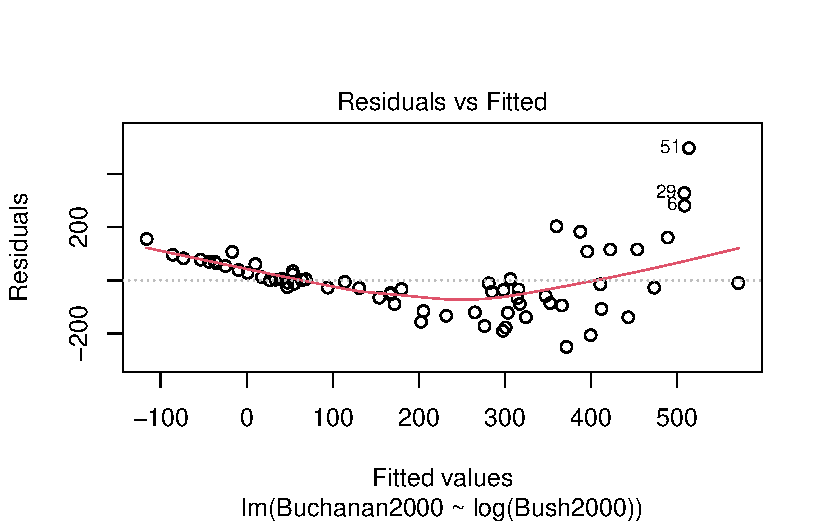
\includegraphics{case_study_1_files/figure-pdf/unnamed-chunk-3-7.pdf}

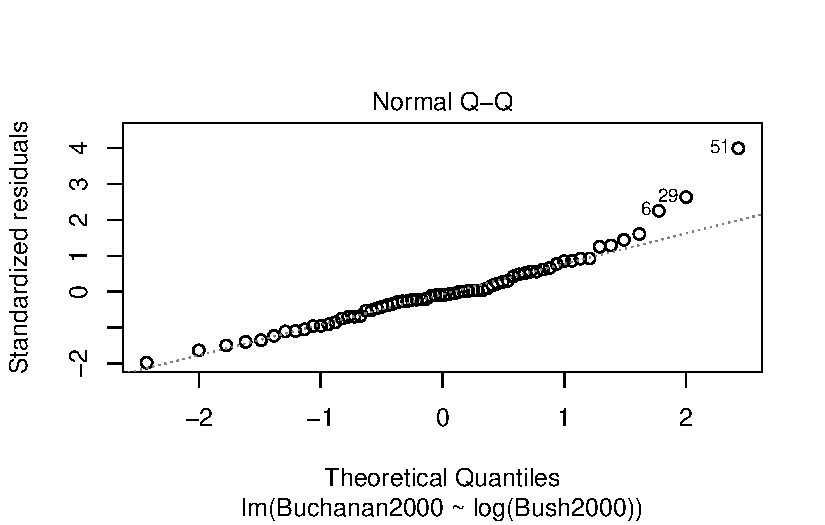
\includegraphics{case_study_1_files/figure-pdf/unnamed-chunk-3-8.pdf}

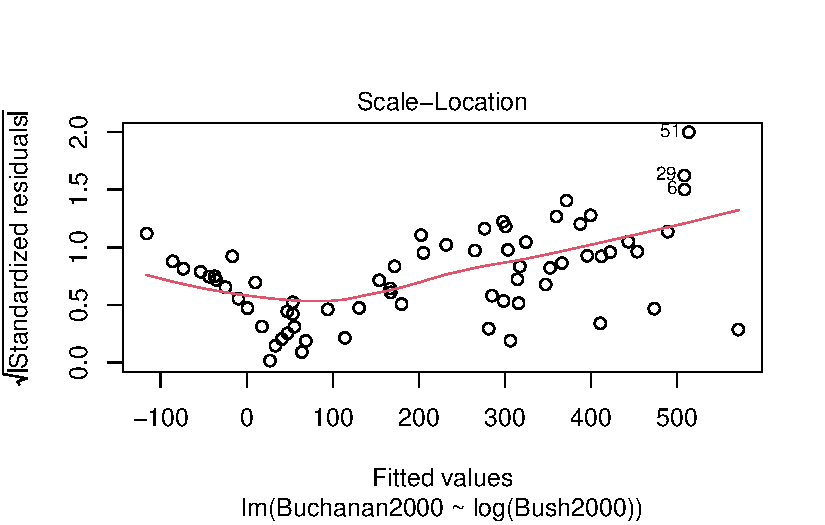
\includegraphics{case_study_1_files/figure-pdf/unnamed-chunk-3-9.pdf}

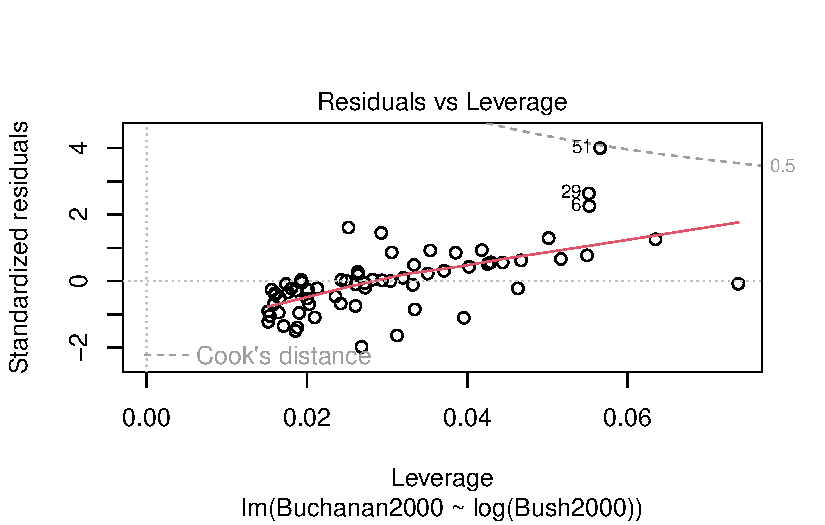
\includegraphics{case_study_1_files/figure-pdf/unnamed-chunk-3-10.pdf}

\begin{Shaded}
\begin{Highlighting}[]
\CommentTok{\# Model with a logarithmic response variable transformation}
\NormalTok{ytransformed }\OtherTok{\textless{}{-}} \FunctionTok{lm}\NormalTok{(}\FunctionTok{log}\NormalTok{(Buchanan2000) }\SpecialCharTok{\textasciitilde{}}\NormalTok{ Bush2000, }\AttributeTok{data =}\NormalTok{ election\_wo\_pb)}
\FunctionTok{plot}\NormalTok{(ytransformed)}
\end{Highlighting}
\end{Shaded}

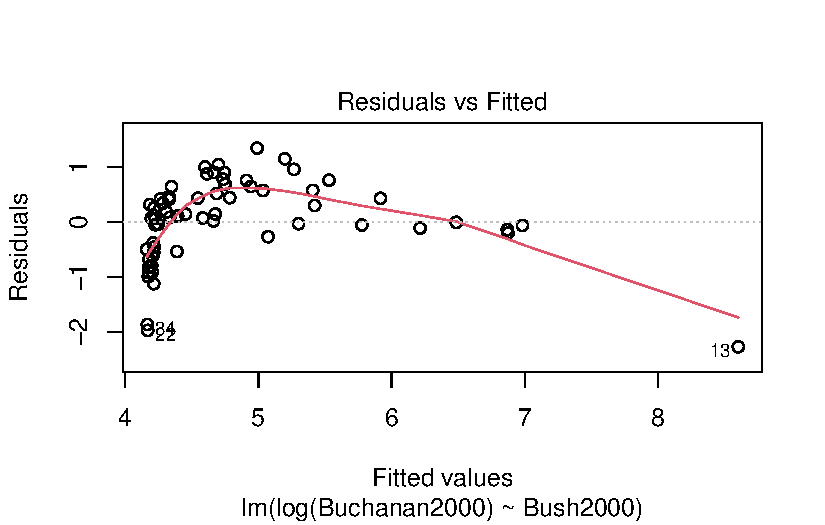
\includegraphics{case_study_1_files/figure-pdf/unnamed-chunk-3-11.pdf}

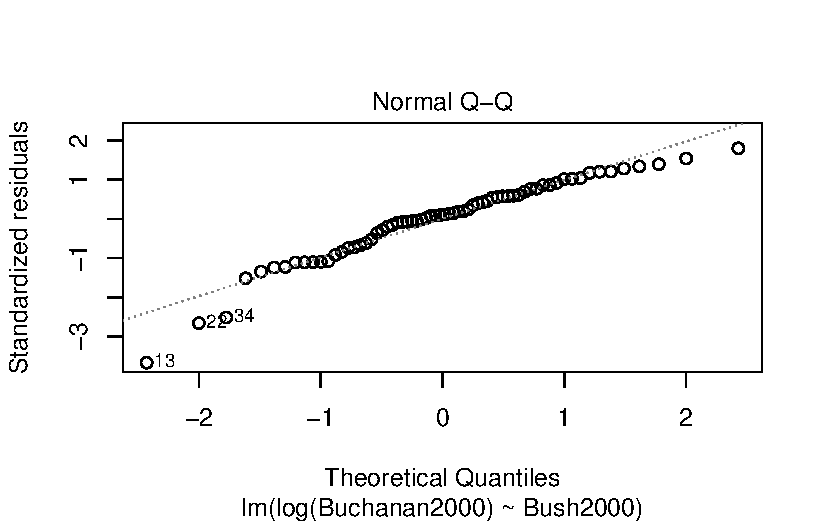
\includegraphics{case_study_1_files/figure-pdf/unnamed-chunk-3-12.pdf}

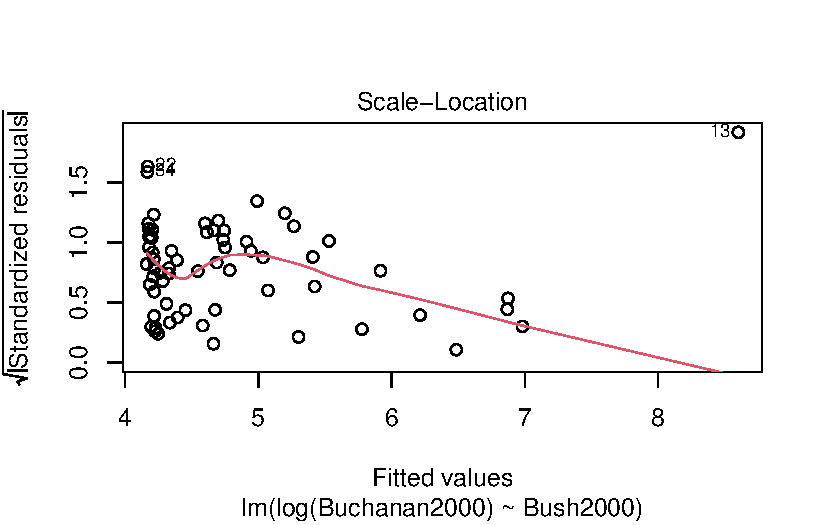
\includegraphics{case_study_1_files/figure-pdf/unnamed-chunk-3-13.pdf}

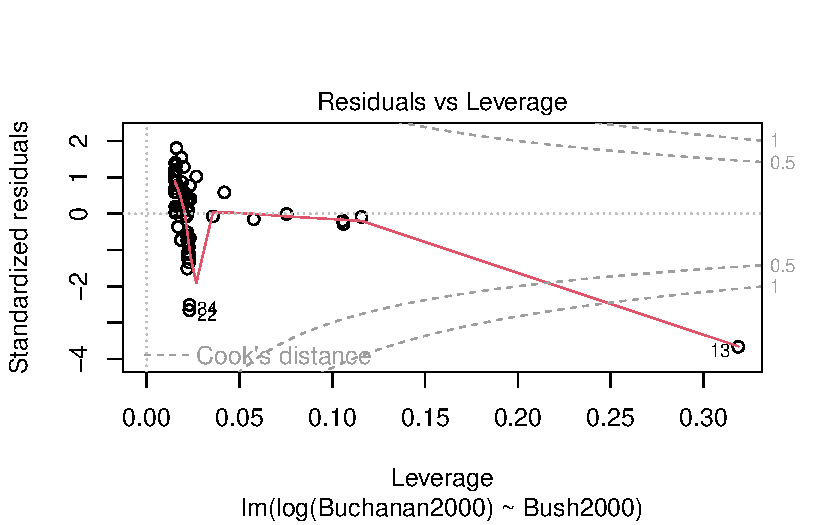
\includegraphics{case_study_1_files/figure-pdf/unnamed-chunk-3-14.pdf}

\begin{Shaded}
\begin{Highlighting}[]
\CommentTok{\# Model with a logarithmic explanatory and response variable transformation}
\NormalTok{both\_transformed }\OtherTok{\textless{}{-}} \FunctionTok{lm}\NormalTok{(}\FunctionTok{log}\NormalTok{(Buchanan2000) }\SpecialCharTok{\textasciitilde{}} \FunctionTok{log}\NormalTok{(Bush2000), }\AttributeTok{data =}\NormalTok{ election\_wo\_pb)}

\CommentTok{\# Getting the coefficients for the doubly transformed model}
\NormalTok{both\_transformed\_table }\OtherTok{\textless{}{-}} \FunctionTok{summary}\NormalTok{(both\_transformed)}\SpecialCharTok{$}\NormalTok{coefficients}

\CommentTok{\# Creating a visible, clean table to display the coefficients from the doubly transformed model}
\NormalTok{both\_transformed\_table }\SpecialCharTok{|\textgreater{}} \FunctionTok{kbl}\NormalTok{(}\AttributeTok{col.names =} \FunctionTok{c}\NormalTok{(}\StringTok{"Estimate"}\NormalTok{, }\StringTok{"Std. Error"}\NormalTok{, }\StringTok{"t value"}\NormalTok{, }\StringTok{"Pr(\textgreater{}|t|)"}\NormalTok{), }\AttributeTok{align =} \StringTok{"c"}\NormalTok{, }\AttributeTok{booktabs =}\NormalTok{ T, }\AttributeTok{linesep=}\StringTok{""}\NormalTok{, }\AttributeTok{digits =} \FunctionTok{c}\NormalTok{(}\DecValTok{2}\NormalTok{, }\DecValTok{2}\NormalTok{, }\DecValTok{2}\NormalTok{, }\DecValTok{4}\NormalTok{)) }\SpecialCharTok{|\textgreater{}} \FunctionTok{kable\_classic}\NormalTok{(}\AttributeTok{full\_width =}\NormalTok{ F, }\AttributeTok{latex\_options =} \FunctionTok{c}\NormalTok{(}\StringTok{"HOLD\_position"}\NormalTok{))}
\end{Highlighting}
\end{Shaded}

\begin{table}[H]
\centering
\begin{tabular}[t]{lcccc}
\toprule
  & Estimate & Std. Error & t value & Pr(>|t|)\\
\midrule
(Intercept) & -2.34 & 0.35 & -6.61 & 0\\
log(Bush2000) & 0.73 & 0.04 & 20.32 & 0\\
\bottomrule
\end{tabular}
\end{table}

\begin{Shaded}
\begin{Highlighting}[]
\FunctionTok{summary}\NormalTok{(both\_transformed)}
\end{Highlighting}
\end{Shaded}

\begin{verbatim}

Call:
lm(formula = log(Buchanan2000) ~ log(Bush2000), data = election_wo_pb)

Residuals:
     Min       1Q   Median       3Q      Max 
-0.95631 -0.21236  0.02503  0.28102  1.02056 

Coefficients:
              Estimate Std. Error t value Pr(>|t|)    
(Intercept)   -2.34149    0.35442  -6.607 9.07e-09 ***
log(Bush2000)  0.73096    0.03597  20.323  < 2e-16 ***
---
Signif. codes:  0 '***' 0.001 '**' 0.01 '*' 0.05 '.' 0.1 ' ' 1

Residual standard error: 0.4198 on 64 degrees of freedom
Multiple R-squared:  0.8658,    Adjusted R-squared:  0.8637 
F-statistic:   413 on 1 and 64 DF,  p-value: < 2.2e-16
\end{verbatim}

\begin{Shaded}
\begin{Highlighting}[]
\CommentTok{\# Creating a prediction interval}
\NormalTok{predicted\_palm\_beach }\OtherTok{=} \FunctionTok{data.frame}\NormalTok{(}\AttributeTok{Bush2000 =} \DecValTok{152846}\NormalTok{)}
\NormalTok{both\_transformed }\SpecialCharTok{|\textgreater{}} \FunctionTok{augment}\NormalTok{(}\AttributeTok{newdata =}\NormalTok{ predicted\_palm\_beach, }\AttributeTok{interval =} \StringTok{"prediction"}\NormalTok{, }\AttributeTok{conf.level =} \FloatTok{0.95}\NormalTok{)}
\end{Highlighting}
\end{Shaded}

\begin{verbatim}
# A tibble: 1 x 4
  Bush2000 .fitted .lower .upper
     <dbl>   <dbl>  <dbl>  <dbl>
1   152846    6.38   5.52   7.24
\end{verbatim}




\end{document}
